Одним из наиболее эффективных подходов к сбору данных является обращение к международным сайтам исследователей, содержащих большое число структурированные данных. 
К сожалению, большинство из них представлены на китайском и английский языках. Для их адаптации был
предложен подход, использующий большие языковые модели в качестве средства перевода на русский язык.
Для этого был использован открытый языковой ассистент llama3 \cite{llamatouvron2023}, владеющий более чем ста языками мира и
имеющий высокие показатели понимания естественного языка.

Перевод 7500 задач с английского и китайского выполнялся в течении 12 часов. 
Полученные результаты приведены в виде таблицы в репозитории\footnote{\url{https://huggingface.co/datasets/NMashalov/olympiad_task_translation}}.
Исследование демонстрирует важность выбора оптимальной инструкции для модели. В отсутствие четких требований модель
нарушает формат постановки задачи, искажает числа и обозначения в ответах. Таким образом, проведенный машинный перевод
требует экспертной адаптации в силу отсутствия явной системны в ошибках. Тем не менее такой подход позволяет 
существенно сократить время перевода в сравнении с работой со словарем, поскольку суть задачи передается моделью верно.  

Цифровые документы также могут быть использованы не только для сбора текста, но и еще для составления аннотированных 
образовательных иллюстраций. Такие данные особенно ценны для больших языковых моделей, обученных работать с изображениями.

Для выделения иллюстраций и подписей к ним была использована сеть YOLO \cite{redmon2016you}.
Эта архитектура нейронной сети имеет способность эффективно дообучаться на небольших выборках данных, 
что позволяет в краткие сроки достигать удовлетворительных результатов. Для ситуаций, в которых число аннотаций и число изображений на
изображении не совпадало, применялся алгоритм на двудольном графе, направленный на максимизацию числа пар.
 
Для получения обучающей выборки была проведена разметка части корпуса цифровых учебников.
Каждое изображение включает в себя текстовую информацию, а также различные чертежи и формулы, характерные для данной области знаний.

\begin{figure}[h]
    \centering
    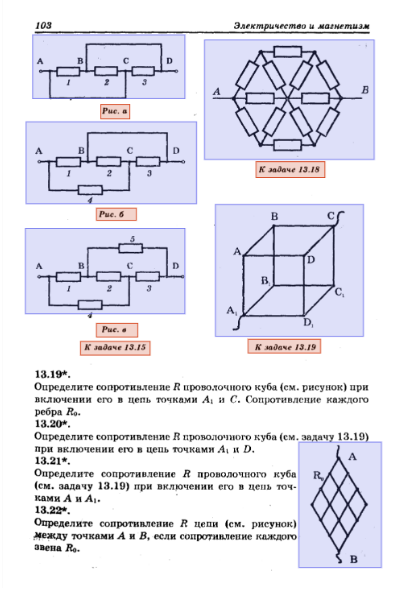
\includegraphics[width=0.5\textwidth]{assets/work/dataset/kirik_labeling.png}
    \caption{Пример аннотированной иллюстрации из книги Генденштейн, Кирик, Гельфгат: 1001 задача по физике}
    \label{annotation}
\end{figure}

Для расширения корпуса и обеспечения его разнообразия была применена аугментация данных. Применялись повороты, масштабирование, изменение освещения и отражение.
Это позволило создать дополнительные вариации входных данных, что способствовало увеличению разнообразия обучающей выборки и повышению устойчивости модели к 
различным вариациям данных. В реальных условиях это определяет эффективность модели при работе с различными вариантами верстки.

Метрическая оценка результатов выделения иллюстрации и аннотации: 

\begin{center}
    \begin{tabular}{||c | c | c||} 
     \hline
     \text{Параметр} & \text{Обучение} & \text{Валидация} \\
     \hline\hline
     \text{mAp} & 78.4 & 75.4  \\ 
     \hline
     \text{“изображение-аннотация”}  & 75.2 & 72.0 \\
     \hline
    \end{tabular}
\end{center}

